% Copyright © 2013 Martin Ueding <dev@martin-ueding.de>
%
% Copyright © 2012-2013 Martin Ueding <dev@martin-ueding.de>

% This is my general purpose LaTeX header file for writing German documents.
% Ideally, you include this using a simple ``% Copyright © 2012-2013 Martin Ueding <dev@martin-ueding.de>

% This is my general purpose LaTeX header file for writing German documents.
% Ideally, you include this using a simple ``% Copyright © 2012-2013 Martin Ueding <dev@martin-ueding.de>

% This is my general purpose LaTeX header file for writing German documents.
% Ideally, you include this using a simple ``\input{header.tex}`` in your main
% document and start with ``\title`` and ``\begin{document}`` afterwards.

% If you need to add additional packages, I recommend not doing this in this
% file, but in your main document. That way, you can just drop in a new
% ``header.tex`` and get all the new commands without having to merge manually.

% Since this file encorporates a CC-BY-SA fragment, this whole files is
% licensed under the CC-BY-SA license.

\documentclass[11pt, ngerman, fleqn, DIV=15, headinclude]{scrartcl}

\usepackage{graphicx}

% Environment to quote the problem. Currently, this is just a new name for the
% quote environment.
\newenvironment{problem}{\begin{quote}}{\end{quote}}

%%%%%%%%%%%%%%%%%%%%%%%%%%%%%%%%%%%%%%%%%%%%%%%%%%%%%%%%%%%%%%%%%%%%%%%%%%%%%%%
%                                Locale, date                                 %
%%%%%%%%%%%%%%%%%%%%%%%%%%%%%%%%%%%%%%%%%%%%%%%%%%%%%%%%%%%%%%%%%%%%%%%%%%%%%%%

\usepackage{babel}
\usepackage[iso]{isodate}

%%%%%%%%%%%%%%%%%%%%%%%%%%%%%%%%%%%%%%%%%%%%%%%%%%%%%%%%%%%%%%%%%%%%%%%%%%%%%%%
%                          Margins and other spacing                          %
%%%%%%%%%%%%%%%%%%%%%%%%%%%%%%%%%%%%%%%%%%%%%%%%%%%%%%%%%%%%%%%%%%%%%%%%%%%%%%%

\usepackage[parfill]{parskip}
\usepackage{setspace}
\usepackage[activate]{microtype}

\setlength{\columnsep}{2cm}

%%%%%%%%%%%%%%%%%%%%%%%%%%%%%%%%%%%%%%%%%%%%%%%%%%%%%%%%%%%%%%%%%%%%%%%%%%%%%%%
%                                    Color                                    %
%%%%%%%%%%%%%%%%%%%%%%%%%%%%%%%%%%%%%%%%%%%%%%%%%%%%%%%%%%%%%%%%%%%%%%%%%%%%%%%

\usepackage[usenames, dvipsnames]{xcolor}

\colorlet{darkred}{red!70!black}
\colorlet{darkblue}{blue!70!black}
\colorlet{darkgreen}{green!40!black}

%%%%%%%%%%%%%%%%%%%%%%%%%%%%%%%%%%%%%%%%%%%%%%%%%%%%%%%%%%%%%%%%%%%%%%%%%%%%%%%
%                         Font and font like settings                         %
%%%%%%%%%%%%%%%%%%%%%%%%%%%%%%%%%%%%%%%%%%%%%%%%%%%%%%%%%%%%%%%%%%%%%%%%%%%%%%%

% This replaces all fonts with Bitstream Charter, Bitstream Vera Sans and
% Bitstream Vera Mono. Math will be rendered in Charter.
\usepackage[charter, greekuppercase=italicized]{mathdesign}
\usepackage{beramono}
\usepackage{berasans}

% Bold, sans-serif tensors. This fragment is taken from “egreg” from
% http://tex.stackexchange.com/a/82747/8945 and licensed under `CC-BY-SA
% <https://creativecommons.org/licenses/by-sa/3.0/>`_.
\usepackage{bm}
\DeclareMathAlphabet{\mathsfit}{\encodingdefault}{\sfdefault}{m}{sl}
\SetMathAlphabet{\mathsfit}{bold}{\encodingdefault}{\sfdefault}{bx}{sl}
\newcommand{\tens}[1]{\bm{\mathsfit{#1}}}

% Bold vectors.
\renewcommand{\vec}[1]{\boldsymbol{#1}}

%%%%%%%%%%%%%%%%%%%%%%%%%%%%%%%%%%%%%%%%%%%%%%%%%%%%%%%%%%%%%%%%%%%%%%%%%%%%%%%
%                               Input encoding                                %
%%%%%%%%%%%%%%%%%%%%%%%%%%%%%%%%%%%%%%%%%%%%%%%%%%%%%%%%%%%%%%%%%%%%%%%%%%%%%%%

\usepackage[T1]{fontenc}
\usepackage[utf8]{inputenc}

%%%%%%%%%%%%%%%%%%%%%%%%%%%%%%%%%%%%%%%%%%%%%%%%%%%%%%%%%%%%%%%%%%%%%%%%%%%%%%%
%                         Hyperrefs and PDF metadata                          %
%%%%%%%%%%%%%%%%%%%%%%%%%%%%%%%%%%%%%%%%%%%%%%%%%%%%%%%%%%%%%%%%%%%%%%%%%%%%%%%

\usepackage{hyperref}
\usepackage{lastpage}

% This sets the author in the properties of the PDF as well. If you want to
% change it, just override it with another ``\hypersetup`` call.
\hypersetup{
	breaklinks=false,
	citecolor=darkgreen,
	colorlinks=true,
	linkcolor=darkblue,
	menucolor=black,
	pdfauthor={Martin Ueding},
	urlcolor=darkblue,
}

%%%%%%%%%%%%%%%%%%%%%%%%%%%%%%%%%%%%%%%%%%%%%%%%%%%%%%%%%%%%%%%%%%%%%%%%%%%%%%%
%                               Math Operators                                %
%%%%%%%%%%%%%%%%%%%%%%%%%%%%%%%%%%%%%%%%%%%%%%%%%%%%%%%%%%%%%%%%%%%%%%%%%%%%%%%

% AMS environments like ``align`` and theorems like ``proof``.
\usepackage{amsmath}
\usepackage{amsthm}

% Common math constructs like partial derivatives.
\usepackage{commath}

% Physical units.
\usepackage[output-decimal-marker={,}]{siunitx}

% Word like operators.
\DeclareMathOperator{\acosh}{arcosh}
\DeclareMathOperator{\arcosh}{arcosh}
\DeclareMathOperator{\arcsinh}{arsinh}
\DeclareMathOperator{\arsinh}{arsinh}
\DeclareMathOperator{\asinh}{arsinh}
\DeclareMathOperator{\card}{card}
\DeclareMathOperator{\csch}{cshs}
\DeclareMathOperator{\diam}{diam}
\DeclareMathOperator{\sech}{sech}
\renewcommand{\Im}{\mathop{{}\mathrm{Im}}\nolimits}
\renewcommand{\Re}{\mathop{{}\mathrm{Re}}\nolimits}

% Fourier transform.
\DeclareMathOperator{\fourier}{\ensuremath{\mathcal{F}}}

% Roman versions of “e” and “i” to serve as Euler's number and the imaginary
% constant.
\newcommand{\ee}{\eup}
\newcommand{\eup}{\mathrm e}
\newcommand{\ii}{\iup}
\newcommand{\iup}{\mathrm i}

% Symbols for the various mathematical fields (natural numbers, integers,
% rational numbers, real numbers, complex numbers).
\newcommand{\C}{\ensuremath{\mathbb C}}
\newcommand{\N}{\ensuremath{\mathbb N}}
\newcommand{\Q}{\ensuremath{\mathbb Q}}
\newcommand{\R}{\ensuremath{\mathbb R}}
\newcommand{\Z}{\ensuremath{\mathbb Z}}

% Shape like operators.
\DeclareMathOperator{\dalambert}{\Box}
\DeclareMathOperator{\laplace}{\bigtriangleup}
\newcommand{\curl}{\vnabla \times}
\newcommand{\divergence}[1]{\inner{\vnabla}{#1}}
\newcommand{\vnabla}{\vec \nabla}

\newcommand{\half}{\frac 12}

% Unit vector (German „Einheitsvektor“).
\newcommand{\ev}{\hat{\vec e}}

% Scientific notation for large numbers.
\newcommand{\e}[1]{\cdot 10^{#1}}

% Mathematician's notation for the inner (scalar, dot) product.
\newcommand{\bracket}[1]{\left\langle #1 \right\rangle}
\newcommand{\inner}[2]{\bracket{#1, #2}}

% Placeholders.
\newcommand{\emesswert}{\del{\messwert \pm \messwert}}
\newcommand{\fehlt}{\textcolor{darkred}{Hier fehlen noch Inhalte.}}
\newcommand{\messwert}{\textcolor{blue}{\square}}
\newcommand{\punkte}{\phantom{xxxxx}}
\newcommand{\punktevon}[1]{\begin{flushright}/ #1\end{flushright}}

% Separator for equations on a single line.
\newcommand{\eqnsep}{,\quad}

% Quantum Mechanics
\newcommand{\braket}[2]{\left\langle #1 \left. \vphantom{#1 #2} \right| #2 \right\rangle}
\newcommand{\braopket}[3]{\left\langle #1 \left. \vphantom{#1 #2 #3} \right| #2 \left. \vphantom{#1 #2 #3} \right| #3 \right\rangle}
\newcommand{\bra}[1]{\left\langle #1 \right|}
\newcommand{\ketbra}[2]{\left| #1 \vphantom{#2} \right\rangle \left\langle #2  \vphantom{#1} \right|}
\newcommand{\ket}[1]{\left| #1 \right\rangle}

%%%%%%%%%%%%%%%%%%%%%%%%%%%%%%%%%%%%%%%%%%%%%%%%%%%%%%%%%%%%%%%%%%%%%%%%%%%%%%%
%                                  Headings                                   %
%%%%%%%%%%%%%%%%%%%%%%%%%%%%%%%%%%%%%%%%%%%%%%%%%%%%%%%%%%%%%%%%%%%%%%%%%%%%%%%

% This will set fancy headings to the top of the page. The page number will be
% accompanied by the total number of pages. That way, you will know if any page
% is missing.
%
% If you do not want this for your document, you can just use
% ``\pagestyle{plain}``.

\usepackage{scrpage2}

\pagestyle{scrheadings}
\automark{section}
\cfoot{\footnotesize{Seite \thepage\ / \pageref{LastPage}}}
\chead{}
\ihead{}
\ohead{\rightmark}
\setheadsepline{.4pt}

%%%%%%%%%%%%%%%%%%%%%%%%%%%%%%%%%%%%%%%%%%%%%%%%%%%%%%%%%%%%%%%%%%%%%%%%%%%%%%%
%                            Bibliography (BibTeX)                            %
%%%%%%%%%%%%%%%%%%%%%%%%%%%%%%%%%%%%%%%%%%%%%%%%%%%%%%%%%%%%%%%%%%%%%%%%%%%%%%%

\newcommand{\bibliographyfile}{../../zentrale_BibTeX/Central}
\bibliographystyle{apalike2}

%%%%%%%%%%%%%%%%%%%%%%%%%%%%%%%%%%%%%%%%%%%%%%%%%%%%%%%%%%%%%%%%%%%%%%%%%%%%%%%
%                                Abbreviations                                %
%%%%%%%%%%%%%%%%%%%%%%%%%%%%%%%%%%%%%%%%%%%%%%%%%%%%%%%%%%%%%%%%%%%%%%%%%%%%%%%

\newcommand{\dhabk}{\mbox{d.\,h.}}

%%%%%%%%%%%%%%%%%%%%%%%%%%%%%%%%%%%%%%%%%%%%%%%%%%%%%%%%%%%%%%%%%%%%%%%%%%%%%%%
%                                  Licences                                   %
%%%%%%%%%%%%%%%%%%%%%%%%%%%%%%%%%%%%%%%%%%%%%%%%%%%%%%%%%%%%%%%%%%%%%%%%%%%%%%%

\usepackage{ccicons}

\newcommand{\ccbysadetext}{%
	\begin{small}
		Dieses Werk bzw. Inhalt steht unter einer
		\href{http://creativecommons.org/licenses/by-sa/3.0/deed.de}{%
			Creative Commons Namensnennung - Weitergabe unter gleichen
		Bedingungen 3.0 Unported Lizenz}.
	\end{small}
}

\newcommand{\ccbysadetitle}{%
	Lizenz: \href{http://creativecommons.org/licenses/by-sa/3.0/deed.de}
	{CC-BY-SA 3.0 \ccbysa}
}
`` in your main
% document and start with ``\title`` and ``\begin{document}`` afterwards.

% If you need to add additional packages, I recommend not doing this in this
% file, but in your main document. That way, you can just drop in a new
% ``header.tex`` and get all the new commands without having to merge manually.

% Since this file encorporates a CC-BY-SA fragment, this whole files is
% licensed under the CC-BY-SA license.

\documentclass[11pt, ngerman, fleqn, DIV=15, headinclude]{scrartcl}

\usepackage{graphicx}

% Environment to quote the problem. Currently, this is just a new name for the
% quote environment.
\newenvironment{problem}{\begin{quote}}{\end{quote}}

%%%%%%%%%%%%%%%%%%%%%%%%%%%%%%%%%%%%%%%%%%%%%%%%%%%%%%%%%%%%%%%%%%%%%%%%%%%%%%%
%                                Locale, date                                 %
%%%%%%%%%%%%%%%%%%%%%%%%%%%%%%%%%%%%%%%%%%%%%%%%%%%%%%%%%%%%%%%%%%%%%%%%%%%%%%%

\usepackage{babel}
\usepackage[iso]{isodate}

%%%%%%%%%%%%%%%%%%%%%%%%%%%%%%%%%%%%%%%%%%%%%%%%%%%%%%%%%%%%%%%%%%%%%%%%%%%%%%%
%                          Margins and other spacing                          %
%%%%%%%%%%%%%%%%%%%%%%%%%%%%%%%%%%%%%%%%%%%%%%%%%%%%%%%%%%%%%%%%%%%%%%%%%%%%%%%

\usepackage[parfill]{parskip}
\usepackage{setspace}
\usepackage[activate]{microtype}

\setlength{\columnsep}{2cm}

%%%%%%%%%%%%%%%%%%%%%%%%%%%%%%%%%%%%%%%%%%%%%%%%%%%%%%%%%%%%%%%%%%%%%%%%%%%%%%%
%                                    Color                                    %
%%%%%%%%%%%%%%%%%%%%%%%%%%%%%%%%%%%%%%%%%%%%%%%%%%%%%%%%%%%%%%%%%%%%%%%%%%%%%%%

\usepackage[usenames, dvipsnames]{xcolor}

\colorlet{darkred}{red!70!black}
\colorlet{darkblue}{blue!70!black}
\colorlet{darkgreen}{green!40!black}

%%%%%%%%%%%%%%%%%%%%%%%%%%%%%%%%%%%%%%%%%%%%%%%%%%%%%%%%%%%%%%%%%%%%%%%%%%%%%%%
%                         Font and font like settings                         %
%%%%%%%%%%%%%%%%%%%%%%%%%%%%%%%%%%%%%%%%%%%%%%%%%%%%%%%%%%%%%%%%%%%%%%%%%%%%%%%

% This replaces all fonts with Bitstream Charter, Bitstream Vera Sans and
% Bitstream Vera Mono. Math will be rendered in Charter.
\usepackage[charter, greekuppercase=italicized]{mathdesign}
\usepackage{beramono}
\usepackage{berasans}

% Bold, sans-serif tensors. This fragment is taken from “egreg” from
% http://tex.stackexchange.com/a/82747/8945 and licensed under `CC-BY-SA
% <https://creativecommons.org/licenses/by-sa/3.0/>`_.
\usepackage{bm}
\DeclareMathAlphabet{\mathsfit}{\encodingdefault}{\sfdefault}{m}{sl}
\SetMathAlphabet{\mathsfit}{bold}{\encodingdefault}{\sfdefault}{bx}{sl}
\newcommand{\tens}[1]{\bm{\mathsfit{#1}}}

% Bold vectors.
\renewcommand{\vec}[1]{\boldsymbol{#1}}

%%%%%%%%%%%%%%%%%%%%%%%%%%%%%%%%%%%%%%%%%%%%%%%%%%%%%%%%%%%%%%%%%%%%%%%%%%%%%%%
%                               Input encoding                                %
%%%%%%%%%%%%%%%%%%%%%%%%%%%%%%%%%%%%%%%%%%%%%%%%%%%%%%%%%%%%%%%%%%%%%%%%%%%%%%%

\usepackage[T1]{fontenc}
\usepackage[utf8]{inputenc}

%%%%%%%%%%%%%%%%%%%%%%%%%%%%%%%%%%%%%%%%%%%%%%%%%%%%%%%%%%%%%%%%%%%%%%%%%%%%%%%
%                         Hyperrefs and PDF metadata                          %
%%%%%%%%%%%%%%%%%%%%%%%%%%%%%%%%%%%%%%%%%%%%%%%%%%%%%%%%%%%%%%%%%%%%%%%%%%%%%%%

\usepackage{hyperref}
\usepackage{lastpage}

% This sets the author in the properties of the PDF as well. If you want to
% change it, just override it with another ``\hypersetup`` call.
\hypersetup{
	breaklinks=false,
	citecolor=darkgreen,
	colorlinks=true,
	linkcolor=darkblue,
	menucolor=black,
	pdfauthor={Martin Ueding},
	urlcolor=darkblue,
}

%%%%%%%%%%%%%%%%%%%%%%%%%%%%%%%%%%%%%%%%%%%%%%%%%%%%%%%%%%%%%%%%%%%%%%%%%%%%%%%
%                               Math Operators                                %
%%%%%%%%%%%%%%%%%%%%%%%%%%%%%%%%%%%%%%%%%%%%%%%%%%%%%%%%%%%%%%%%%%%%%%%%%%%%%%%

% AMS environments like ``align`` and theorems like ``proof``.
\usepackage{amsmath}
\usepackage{amsthm}

% Common math constructs like partial derivatives.
\usepackage{commath}

% Physical units.
\usepackage[output-decimal-marker={,}]{siunitx}

% Word like operators.
\DeclareMathOperator{\acosh}{arcosh}
\DeclareMathOperator{\arcosh}{arcosh}
\DeclareMathOperator{\arcsinh}{arsinh}
\DeclareMathOperator{\arsinh}{arsinh}
\DeclareMathOperator{\asinh}{arsinh}
\DeclareMathOperator{\card}{card}
\DeclareMathOperator{\csch}{cshs}
\DeclareMathOperator{\diam}{diam}
\DeclareMathOperator{\sech}{sech}
\renewcommand{\Im}{\mathop{{}\mathrm{Im}}\nolimits}
\renewcommand{\Re}{\mathop{{}\mathrm{Re}}\nolimits}

% Fourier transform.
\DeclareMathOperator{\fourier}{\ensuremath{\mathcal{F}}}

% Roman versions of “e” and “i” to serve as Euler's number and the imaginary
% constant.
\newcommand{\ee}{\eup}
\newcommand{\eup}{\mathrm e}
\newcommand{\ii}{\iup}
\newcommand{\iup}{\mathrm i}

% Symbols for the various mathematical fields (natural numbers, integers,
% rational numbers, real numbers, complex numbers).
\newcommand{\C}{\ensuremath{\mathbb C}}
\newcommand{\N}{\ensuremath{\mathbb N}}
\newcommand{\Q}{\ensuremath{\mathbb Q}}
\newcommand{\R}{\ensuremath{\mathbb R}}
\newcommand{\Z}{\ensuremath{\mathbb Z}}

% Shape like operators.
\DeclareMathOperator{\dalambert}{\Box}
\DeclareMathOperator{\laplace}{\bigtriangleup}
\newcommand{\curl}{\vnabla \times}
\newcommand{\divergence}[1]{\inner{\vnabla}{#1}}
\newcommand{\vnabla}{\vec \nabla}

\newcommand{\half}{\frac 12}

% Unit vector (German „Einheitsvektor“).
\newcommand{\ev}{\hat{\vec e}}

% Scientific notation for large numbers.
\newcommand{\e}[1]{\cdot 10^{#1}}

% Mathematician's notation for the inner (scalar, dot) product.
\newcommand{\bracket}[1]{\left\langle #1 \right\rangle}
\newcommand{\inner}[2]{\bracket{#1, #2}}

% Placeholders.
\newcommand{\emesswert}{\del{\messwert \pm \messwert}}
\newcommand{\fehlt}{\textcolor{darkred}{Hier fehlen noch Inhalte.}}
\newcommand{\messwert}{\textcolor{blue}{\square}}
\newcommand{\punkte}{\phantom{xxxxx}}
\newcommand{\punktevon}[1]{\begin{flushright}/ #1\end{flushright}}

% Separator for equations on a single line.
\newcommand{\eqnsep}{,\quad}

% Quantum Mechanics
\newcommand{\braket}[2]{\left\langle #1 \left. \vphantom{#1 #2} \right| #2 \right\rangle}
\newcommand{\braopket}[3]{\left\langle #1 \left. \vphantom{#1 #2 #3} \right| #2 \left. \vphantom{#1 #2 #3} \right| #3 \right\rangle}
\newcommand{\bra}[1]{\left\langle #1 \right|}
\newcommand{\ketbra}[2]{\left| #1 \vphantom{#2} \right\rangle \left\langle #2  \vphantom{#1} \right|}
\newcommand{\ket}[1]{\left| #1 \right\rangle}

%%%%%%%%%%%%%%%%%%%%%%%%%%%%%%%%%%%%%%%%%%%%%%%%%%%%%%%%%%%%%%%%%%%%%%%%%%%%%%%
%                                  Headings                                   %
%%%%%%%%%%%%%%%%%%%%%%%%%%%%%%%%%%%%%%%%%%%%%%%%%%%%%%%%%%%%%%%%%%%%%%%%%%%%%%%

% This will set fancy headings to the top of the page. The page number will be
% accompanied by the total number of pages. That way, you will know if any page
% is missing.
%
% If you do not want this for your document, you can just use
% ``\pagestyle{plain}``.

\usepackage{scrpage2}

\pagestyle{scrheadings}
\automark{section}
\cfoot{\footnotesize{Seite \thepage\ / \pageref{LastPage}}}
\chead{}
\ihead{}
\ohead{\rightmark}
\setheadsepline{.4pt}

%%%%%%%%%%%%%%%%%%%%%%%%%%%%%%%%%%%%%%%%%%%%%%%%%%%%%%%%%%%%%%%%%%%%%%%%%%%%%%%
%                            Bibliography (BibTeX)                            %
%%%%%%%%%%%%%%%%%%%%%%%%%%%%%%%%%%%%%%%%%%%%%%%%%%%%%%%%%%%%%%%%%%%%%%%%%%%%%%%

\newcommand{\bibliographyfile}{../../zentrale_BibTeX/Central}
\bibliographystyle{apalike2}

%%%%%%%%%%%%%%%%%%%%%%%%%%%%%%%%%%%%%%%%%%%%%%%%%%%%%%%%%%%%%%%%%%%%%%%%%%%%%%%
%                                Abbreviations                                %
%%%%%%%%%%%%%%%%%%%%%%%%%%%%%%%%%%%%%%%%%%%%%%%%%%%%%%%%%%%%%%%%%%%%%%%%%%%%%%%

\newcommand{\dhabk}{\mbox{d.\,h.}}

%%%%%%%%%%%%%%%%%%%%%%%%%%%%%%%%%%%%%%%%%%%%%%%%%%%%%%%%%%%%%%%%%%%%%%%%%%%%%%%
%                                  Licences                                   %
%%%%%%%%%%%%%%%%%%%%%%%%%%%%%%%%%%%%%%%%%%%%%%%%%%%%%%%%%%%%%%%%%%%%%%%%%%%%%%%

\usepackage{ccicons}

\newcommand{\ccbysadetext}{%
	\begin{small}
		Dieses Werk bzw. Inhalt steht unter einer
		\href{http://creativecommons.org/licenses/by-sa/3.0/deed.de}{%
			Creative Commons Namensnennung - Weitergabe unter gleichen
		Bedingungen 3.0 Unported Lizenz}.
	\end{small}
}

\newcommand{\ccbysadetitle}{%
	Lizenz: \href{http://creativecommons.org/licenses/by-sa/3.0/deed.de}
	{CC-BY-SA 3.0 \ccbysa}
}
`` in your main
% document and start with ``\title`` and ``\begin{document}`` afterwards.

% If you need to add additional packages, I recommend not doing this in this
% file, but in your main document. That way, you can just drop in a new
% ``header.tex`` and get all the new commands without having to merge manually.

% Since this file encorporates a CC-BY-SA fragment, this whole files is
% licensed under the CC-BY-SA license.

\documentclass[11pt, ngerman, fleqn, DIV=15, headinclude]{scrartcl}

\usepackage{graphicx}

% Environment to quote the problem. Currently, this is just a new name for the
% quote environment.
\newenvironment{problem}{\begin{quote}}{\end{quote}}

%%%%%%%%%%%%%%%%%%%%%%%%%%%%%%%%%%%%%%%%%%%%%%%%%%%%%%%%%%%%%%%%%%%%%%%%%%%%%%%
%                                Locale, date                                 %
%%%%%%%%%%%%%%%%%%%%%%%%%%%%%%%%%%%%%%%%%%%%%%%%%%%%%%%%%%%%%%%%%%%%%%%%%%%%%%%

\usepackage{babel}
\usepackage[iso]{isodate}

%%%%%%%%%%%%%%%%%%%%%%%%%%%%%%%%%%%%%%%%%%%%%%%%%%%%%%%%%%%%%%%%%%%%%%%%%%%%%%%
%                          Margins and other spacing                          %
%%%%%%%%%%%%%%%%%%%%%%%%%%%%%%%%%%%%%%%%%%%%%%%%%%%%%%%%%%%%%%%%%%%%%%%%%%%%%%%

\usepackage[parfill]{parskip}
\usepackage{setspace}
\usepackage[activate]{microtype}

\setlength{\columnsep}{2cm}

%%%%%%%%%%%%%%%%%%%%%%%%%%%%%%%%%%%%%%%%%%%%%%%%%%%%%%%%%%%%%%%%%%%%%%%%%%%%%%%
%                                    Color                                    %
%%%%%%%%%%%%%%%%%%%%%%%%%%%%%%%%%%%%%%%%%%%%%%%%%%%%%%%%%%%%%%%%%%%%%%%%%%%%%%%

\usepackage[usenames, dvipsnames]{xcolor}

\colorlet{darkred}{red!70!black}
\colorlet{darkblue}{blue!70!black}
\colorlet{darkgreen}{green!40!black}

%%%%%%%%%%%%%%%%%%%%%%%%%%%%%%%%%%%%%%%%%%%%%%%%%%%%%%%%%%%%%%%%%%%%%%%%%%%%%%%
%                         Font and font like settings                         %
%%%%%%%%%%%%%%%%%%%%%%%%%%%%%%%%%%%%%%%%%%%%%%%%%%%%%%%%%%%%%%%%%%%%%%%%%%%%%%%

% This replaces all fonts with Bitstream Charter, Bitstream Vera Sans and
% Bitstream Vera Mono. Math will be rendered in Charter.
\usepackage[charter, greekuppercase=italicized]{mathdesign}
\usepackage{beramono}
\usepackage{berasans}

% Bold, sans-serif tensors. This fragment is taken from “egreg” from
% http://tex.stackexchange.com/a/82747/8945 and licensed under `CC-BY-SA
% <https://creativecommons.org/licenses/by-sa/3.0/>`_.
\usepackage{bm}
\DeclareMathAlphabet{\mathsfit}{\encodingdefault}{\sfdefault}{m}{sl}
\SetMathAlphabet{\mathsfit}{bold}{\encodingdefault}{\sfdefault}{bx}{sl}
\newcommand{\tens}[1]{\bm{\mathsfit{#1}}}

% Bold vectors.
\renewcommand{\vec}[1]{\boldsymbol{#1}}

%%%%%%%%%%%%%%%%%%%%%%%%%%%%%%%%%%%%%%%%%%%%%%%%%%%%%%%%%%%%%%%%%%%%%%%%%%%%%%%
%                               Input encoding                                %
%%%%%%%%%%%%%%%%%%%%%%%%%%%%%%%%%%%%%%%%%%%%%%%%%%%%%%%%%%%%%%%%%%%%%%%%%%%%%%%

\usepackage[T1]{fontenc}
\usepackage[utf8]{inputenc}

%%%%%%%%%%%%%%%%%%%%%%%%%%%%%%%%%%%%%%%%%%%%%%%%%%%%%%%%%%%%%%%%%%%%%%%%%%%%%%%
%                         Hyperrefs and PDF metadata                          %
%%%%%%%%%%%%%%%%%%%%%%%%%%%%%%%%%%%%%%%%%%%%%%%%%%%%%%%%%%%%%%%%%%%%%%%%%%%%%%%

\usepackage{hyperref}
\usepackage{lastpage}

% This sets the author in the properties of the PDF as well. If you want to
% change it, just override it with another ``\hypersetup`` call.
\hypersetup{
	breaklinks=false,
	citecolor=darkgreen,
	colorlinks=true,
	linkcolor=darkblue,
	menucolor=black,
	pdfauthor={Martin Ueding},
	urlcolor=darkblue,
}

%%%%%%%%%%%%%%%%%%%%%%%%%%%%%%%%%%%%%%%%%%%%%%%%%%%%%%%%%%%%%%%%%%%%%%%%%%%%%%%
%                               Math Operators                                %
%%%%%%%%%%%%%%%%%%%%%%%%%%%%%%%%%%%%%%%%%%%%%%%%%%%%%%%%%%%%%%%%%%%%%%%%%%%%%%%

% AMS environments like ``align`` and theorems like ``proof``.
\usepackage{amsmath}
\usepackage{amsthm}

% Common math constructs like partial derivatives.
\usepackage{commath}

% Physical units.
\usepackage[output-decimal-marker={,}]{siunitx}

% Word like operators.
\DeclareMathOperator{\acosh}{arcosh}
\DeclareMathOperator{\arcosh}{arcosh}
\DeclareMathOperator{\arcsinh}{arsinh}
\DeclareMathOperator{\arsinh}{arsinh}
\DeclareMathOperator{\asinh}{arsinh}
\DeclareMathOperator{\card}{card}
\DeclareMathOperator{\csch}{cshs}
\DeclareMathOperator{\diam}{diam}
\DeclareMathOperator{\sech}{sech}
\renewcommand{\Im}{\mathop{{}\mathrm{Im}}\nolimits}
\renewcommand{\Re}{\mathop{{}\mathrm{Re}}\nolimits}

% Fourier transform.
\DeclareMathOperator{\fourier}{\ensuremath{\mathcal{F}}}

% Roman versions of “e” and “i” to serve as Euler's number and the imaginary
% constant.
\newcommand{\ee}{\eup}
\newcommand{\eup}{\mathrm e}
\newcommand{\ii}{\iup}
\newcommand{\iup}{\mathrm i}

% Symbols for the various mathematical fields (natural numbers, integers,
% rational numbers, real numbers, complex numbers).
\newcommand{\C}{\ensuremath{\mathbb C}}
\newcommand{\N}{\ensuremath{\mathbb N}}
\newcommand{\Q}{\ensuremath{\mathbb Q}}
\newcommand{\R}{\ensuremath{\mathbb R}}
\newcommand{\Z}{\ensuremath{\mathbb Z}}

% Shape like operators.
\DeclareMathOperator{\dalambert}{\Box}
\DeclareMathOperator{\laplace}{\bigtriangleup}
\newcommand{\curl}{\vnabla \times}
\newcommand{\divergence}[1]{\inner{\vnabla}{#1}}
\newcommand{\vnabla}{\vec \nabla}

\newcommand{\half}{\frac 12}

% Unit vector (German „Einheitsvektor“).
\newcommand{\ev}{\hat{\vec e}}

% Scientific notation for large numbers.
\newcommand{\e}[1]{\cdot 10^{#1}}

% Mathematician's notation for the inner (scalar, dot) product.
\newcommand{\bracket}[1]{\left\langle #1 \right\rangle}
\newcommand{\inner}[2]{\bracket{#1, #2}}

% Placeholders.
\newcommand{\emesswert}{\del{\messwert \pm \messwert}}
\newcommand{\fehlt}{\textcolor{darkred}{Hier fehlen noch Inhalte.}}
\newcommand{\messwert}{\textcolor{blue}{\square}}
\newcommand{\punkte}{\phantom{xxxxx}}
\newcommand{\punktevon}[1]{\begin{flushright}/ #1\end{flushright}}

% Separator for equations on a single line.
\newcommand{\eqnsep}{,\quad}

% Quantum Mechanics
\newcommand{\braket}[2]{\left\langle #1 \left. \vphantom{#1 #2} \right| #2 \right\rangle}
\newcommand{\braopket}[3]{\left\langle #1 \left. \vphantom{#1 #2 #3} \right| #2 \left. \vphantom{#1 #2 #3} \right| #3 \right\rangle}
\newcommand{\bra}[1]{\left\langle #1 \right|}
\newcommand{\ketbra}[2]{\left| #1 \vphantom{#2} \right\rangle \left\langle #2  \vphantom{#1} \right|}
\newcommand{\ket}[1]{\left| #1 \right\rangle}

%%%%%%%%%%%%%%%%%%%%%%%%%%%%%%%%%%%%%%%%%%%%%%%%%%%%%%%%%%%%%%%%%%%%%%%%%%%%%%%
%                                  Headings                                   %
%%%%%%%%%%%%%%%%%%%%%%%%%%%%%%%%%%%%%%%%%%%%%%%%%%%%%%%%%%%%%%%%%%%%%%%%%%%%%%%

% This will set fancy headings to the top of the page. The page number will be
% accompanied by the total number of pages. That way, you will know if any page
% is missing.
%
% If you do not want this for your document, you can just use
% ``\pagestyle{plain}``.

\usepackage{scrpage2}

\pagestyle{scrheadings}
\automark{section}
\cfoot{\footnotesize{Seite \thepage\ / \pageref{LastPage}}}
\chead{}
\ihead{}
\ohead{\rightmark}
\setheadsepline{.4pt}

%%%%%%%%%%%%%%%%%%%%%%%%%%%%%%%%%%%%%%%%%%%%%%%%%%%%%%%%%%%%%%%%%%%%%%%%%%%%%%%
%                            Bibliography (BibTeX)                            %
%%%%%%%%%%%%%%%%%%%%%%%%%%%%%%%%%%%%%%%%%%%%%%%%%%%%%%%%%%%%%%%%%%%%%%%%%%%%%%%

\newcommand{\bibliographyfile}{../../zentrale_BibTeX/Central}
\bibliographystyle{apalike2}

%%%%%%%%%%%%%%%%%%%%%%%%%%%%%%%%%%%%%%%%%%%%%%%%%%%%%%%%%%%%%%%%%%%%%%%%%%%%%%%
%                                Abbreviations                                %
%%%%%%%%%%%%%%%%%%%%%%%%%%%%%%%%%%%%%%%%%%%%%%%%%%%%%%%%%%%%%%%%%%%%%%%%%%%%%%%

\newcommand{\dhabk}{\mbox{d.\,h.}}

%%%%%%%%%%%%%%%%%%%%%%%%%%%%%%%%%%%%%%%%%%%%%%%%%%%%%%%%%%%%%%%%%%%%%%%%%%%%%%%
%                                  Licences                                   %
%%%%%%%%%%%%%%%%%%%%%%%%%%%%%%%%%%%%%%%%%%%%%%%%%%%%%%%%%%%%%%%%%%%%%%%%%%%%%%%

\usepackage{ccicons}

\newcommand{\ccbysadetext}{%
	\begin{small}
		Dieses Werk bzw. Inhalt steht unter einer
		\href{http://creativecommons.org/licenses/by-sa/3.0/deed.de}{%
			Creative Commons Namensnennung - Weitergabe unter gleichen
		Bedingungen 3.0 Unported Lizenz}.
	\end{small}
}

\newcommand{\ccbysadetitle}{%
	Lizenz: \href{http://creativecommons.org/licenses/by-sa/3.0/deed.de}
	{CC-BY-SA 3.0 \ccbysa}
}


\usepackage{tikz}
\usetikzlibrary{calc}

\newcommand{\themodul}{physik411}
\newcommand{\thegruppe}{Gruppe 2 -- Florian Seidler}
\newcommand{\theuebung}{8}

\ifoot{\footnotesize{Martin Ueding}}
\ihead{\themodul{} -- Übung \theuebung}
\ofoot{\footnotesize{\thegruppe}}

\def\thesubsection{\thesection\alph{subsection}}

\title{\themodul{} -- Übung \theuebung}
\subtitle{\thegruppe}
\author{
	Martin Ueding \footnote{\href{mailto:mu@uni-bonn.de}{mu@uni-bonn.de}}
}

\hypersetup{
	pdftitle={\themodul {} - Übung \theuebung},
}

\begin{document}

\maketitle

\begin{center}
	\ccbysadetitle
\end{center}

\begin{table}[h]
	\centering
	\begin{tabular}{l*3{|c}}
		Aufgabe
		& \ref 1
		& \ref 2
		& $\sum$   \\
		\hline
		Punkte
		& \punkte / 18
		& \punkte / 14
		& \punkte / 32
	\end{tabular}
\end{table}

%%%%%%%%%%%%%%%%%%%%%%%%%%%%%%%%%%%%%%%%%%%%%%%%%%%%%%%%%%%%%%%%%%%%%%%%%%%%%%%
%              Das Morse-Potential eines diatomischen Moleküls               %
%%%%%%%%%%%%%%%%%%%%%%%%%%%%%%%%%%%%%%%%%%%%%%%%%%%%%%%%%%%%%%%%%%%%%%%%%%%%%%%

\section{Das Morse-Potential eines diatomischen Moleküls}
\label 1

\subsection{}

\subsection{}

\subsection{Plot und Größen}

Für verschiedene $\ell$ ist das Morse-Potential in Abbildung \ref{fig:1/c/Plot}
dargestellt.

\begin{figure}
	\centering
	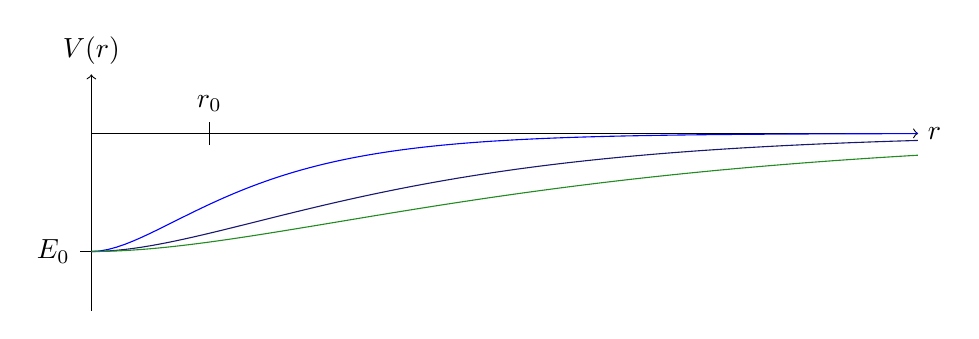
\begin{tikzpicture}[scale=1.5]
		\draw[->] (0, 0) -- ++(7, 0) node[right] {$r$};
		\draw[->] (0, -1.5) -- ++(0, 2) node[above] {$V(r)$};
		\draw (1, -.1) -- ++(0, .2) node[above] {$r_0$};
		\draw (.1, -1) -- ++(-.2, 0) node[left] {$E_0$};
		\draw[domain=0:7, samples=100, color=blue] plot (\x,{(exp(-\x) - 1)^2 - 1});
		\draw[domain=0:7, samples=100, color=MidnightBlue] plot (\x,{(exp(-\x/2) - 1)^2 - 1});
		\draw[domain=0:7, samples=100, color=ForestGreen] plot (\x,{(exp(-\x/3) - 1)^2 - 1});
	\end{tikzpicture}
	\caption{%
		In \textcolor{blue}{blau} das Morse-Potential für $\ell = 1$. In
		\textcolor{MidnightBlue}{mitternachtsblau} den Fall $\ell = 2$. Sowie
		in \textcolor{ForestGreen}{waldgrün} $\ell = 3$.
	}
	\label{fig:1/c/Plot}
\end{figure}

Die Rolle von $\ell$ scheint eine Art charakteristische Länge zu sein. Je
größer $\ell$ ist, desto länger reicht das Potential. Beim Wasserstoff ist dies
ähnlich, da die zugeordneten Laguerrefunktionen mit zunehmendem $\ell$ auch
langreichweitiger werden. Daher ist auch der Quantendefekt bei größeren $\ell$
kleiner, weil sich die Elektronen nicht mehr so häufig am Kern aufhalten.

%%%%%%%%%%%%%%%%%%%%%%%%%%%%%%%%%%%%%%%%%%%%%%%%%%%%%%%%%%%%%%%%%%%%%%%%%%%%%%%
%                                    Ende                                     %
%%%%%%%%%%%%%%%%%%%%%%%%%%%%%%%%%%%%%%%%%%%%%%%%%%%%%%%%%%%%%%%%%%%%%%%%%%%%%%%

\IfFileExists{\bibliographyfile}{
	%\bibliography{\bibliographyfile}
}{}

\end{document}

% vim: spell spelllang=de
